\documentclass{article}
\usepackage{tikz}

\begin{document}

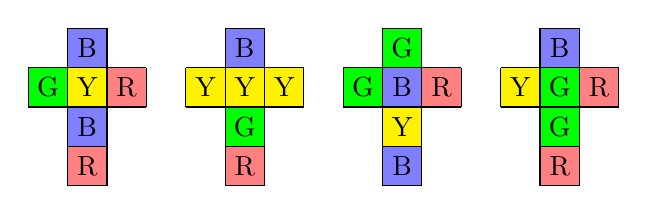
\begin{tikzpicture}[scale=.5]

\fill[red!50!white] (1,0) rectangle (2,1);
\fill[blue!50!white] (1,1) rectangle (2,2);
\fill[yellow] (1,2) rectangle (2,3);
\fill[blue!50!white] (1,3) rectangle (2,4);
\fill[green] (0,2) rectangle (1,3);
\fill[red!50!white] (2,2) rectangle (3,3);
\draw (1.5, .5) node {R};
\draw (2.5, 2.5) node {R};
\draw (1.5, 1.5) node {B};
\draw (1.5, 2.5) node {Y};
\draw (1.5, 3.5) node {B};
\draw (.5, 2.5) node {G};



\draw (1,0) grid (2,4);
\draw (0,2) grid (3,3);


\begin{scope}[xshift=4cm]

\fill[red!50!white] (1,0) rectangle (2,1);
\fill[green] (1,1) rectangle (2,2);

\fill[blue!50!white] (1,3) rectangle (2,4);
\fill[yellow] (0,2) rectangle (3,3);



\draw (1.5, .5) node {R};
\draw (1.5, 1.5) node {G};
\draw (1.5, 2.5) node {Y};
\draw (1.5, 3.5) node {B};
\draw (.5, 2.5) node {Y};
\draw (2.5, 2.5) node {Y};
\draw (1,0) grid (2,4);
\draw (0,2) grid (3,3);
\end{scope}

\begin{scope}[xshift=8cm]

\fill[blue!50!white] (1,0) rectangle (2,1);
\fill[yellow] (1,1) rectangle (2,2);
\fill[blue!50!white] (1,2) rectangle (2,3);
\fill[green] (1,3) rectangle (2,4);
\fill[green] (0,2) rectangle (1,3);
\fill[red!50!white] (2,2) rectangle (3,3);
\draw (1.5, .5) node {B};
\draw (1.5, 1.5) node {Y};
\draw (1.5, 2.5) node {B};
\draw (1.5, 3.5) node {G};
\draw (.5, 2.5) node {G};
\draw (2.5, 2.5) node {R};


\draw (1,0) grid (2,4);
\draw (0,2) grid (3,3);
\end{scope}


\begin{scope}[xshift=12cm]

\fill[red!50!white] (1,0) rectangle (2,1);
\fill[green] (1,1) rectangle (2,2);
\fill[green] (1,2) rectangle (2,3);
\fill[blue!50!white] (1,3) rectangle (2,4);
\fill[yellow] (0,2) rectangle (1,3);
\fill[red!50!white] (2,2) rectangle (3,3);
\draw (1.5, .5) node {R};
\draw (1.5, 1.5) node {G};
\draw (1.5, 2.5) node {G};
\draw (1.5, 3.5) node {B};
\draw (.5, 2.5) node {Y};
\draw (2.5, 2.5) node {R};


\draw (1,0) grid (2,4);
\draw (0,2) grid (3,3);
\end{scope}



\end{tikzpicture}




\begin{tikzpicture} \GraphInit[vstyle=Welsh] \SetGraphUnit{2} \Vertices{circle}{A,B,C,D,E} \SetUpEdge[style={->}] \Edges[label=1](A,B) \Edges[label=1](B,C) \Edges[label=1](C,D) \Edges[label=\$1\$](D,E) \Edges[label=x1](A,C) \Edges[label=x2](A,D) \Edges[label=x3](A,E) \SetVertexNoLabel \end{tikzpicture}

\end{document}
